\documentclass[margin=2mm]{standalone}
\usepackage{pgfplots}
\pgfplotsset{compat=1.16}
\usepackage{tikz}
\usetikzlibrary{3d,calc,shapes}
\begin{document}
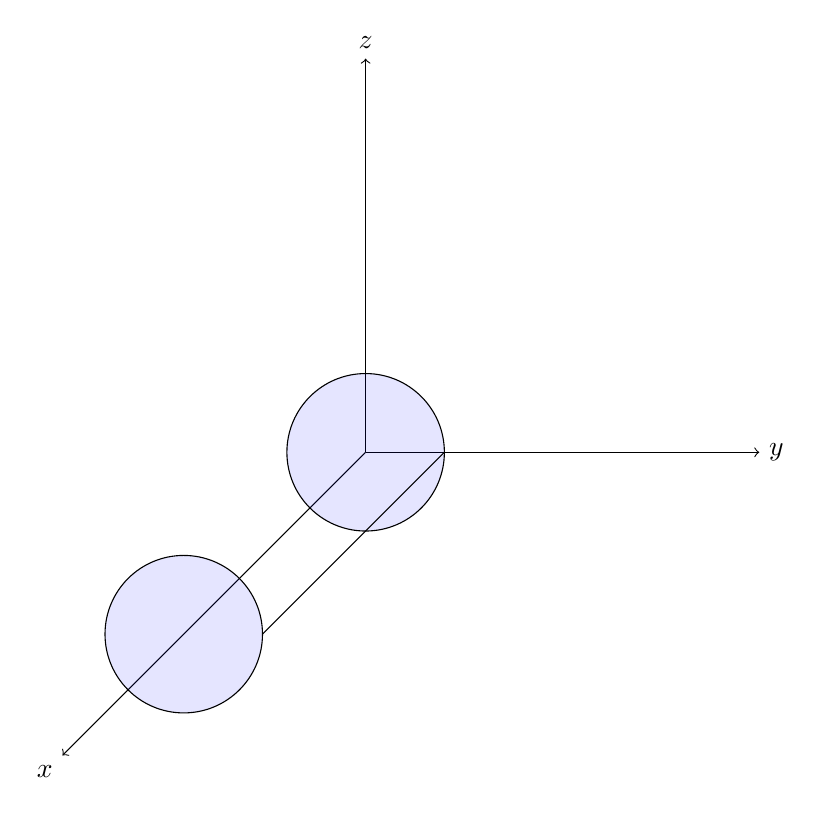
\begin{tikzpicture}
    %coordinate system
    \draw[->] (0,0,0)--++(5,0,0) node[right]{$y$}; %x
    \draw[->] (0,0,0)--++(0,5,0) node[above]{$z$}; %y
    \draw[->] (0,0,0)--++(0,0,10) node[below left]{$x$}; %z

    % cylinder:
    \draw[preaction={fill=blue,very  nearly transparent}](1,0,0)
    arc[start angle=0, end angle=360, radius=1]node[inner sep=0](n11){};

    \draw[preaction={fill=blue,very  nearly transparent}](1,0,6)

    arc[start angle=0, end angle=360, radius=1]node[inner sep=0](n12){};
    \draw (1,0,0) -- (1,0,6);
    %arc[start angle=0, end angle=180, radius=4]node[inner sep=0](n11){};
    % -- ++(0,0,8.5)node[inner sep=0](n21){}
    %arc[start angle=180, end angle=0, radius=4] -- cycle;
    % \draw[](n21.center)--(0,0,8.5)--(4,0,8.5);
    % \draw[](0,4,0)--(n11.center);
\end{tikzpicture}
\end{document}